\documentclass[review]{elsarticle}

\usepackage{lineno,hyperref}
\modulolinenumbers[5]

\usepackage{adjustbox}
\usepackage{amsmath}
\DeclareMathOperator*{\argmax}{arg\,max}
\DeclareMathOperator*{\argmin}{arg\,min}


\journal{Journal of Parallel and Distributed Computing}

%%%%%%%%%%%%%%%%%%%%%%%
%% Elsevier bibliography styles
%%%%%%%%%%%%%%%%%%%%%%%
%% To change the style, put a % in front of the second line of the current style and
%% remove the % from the second line of the style you would like to use.
%%%%%%%%%%%%%%%%%%%%%%%

%% Numbered
%\bibliographystyle{model1-num-names}

%% Numbered without titles
%\bibliographystyle{model1a-num-names}

%% Harvard
%\bibliographystyle{model2-names.bst}\biboptions{authoryear}

%% Vancouver numbered
%\usepackage{numcompress}\bibliographystyle{model3-num-names}

%% Vancouver name/year
%\usepackage{numcompress}\bibliographystyle{model4-names}\biboptions{authoryear}

%% APA style
%\bibliographystyle{model5-names}\biboptions{authoryear}

%% AMA style
%\usepackage{numcompress}\bibliographystyle{model6-num-names}

%% `Elsevier LaTeX' style
\bibliographystyle{elsarticle-num}
%%%%%%%%%%%%%%%%%%%%%%%

\begin{document}

\begin{frontmatter}

\title{Parallel Solving of Multiple Information-Coordinated Global Optimization Problems}

%% Group authors per affiliation:
%\author{Victor Gergel \and Evgeniy Kozinov}
%\address{Lobachevsky State University of Nizhni Novgorod, Nizhni Novgorod, Russia}
%\ead{gergel@unn.ru}

\author[mymainaddress]{Victor Gergel}
\ead{gergel@unn.ru}

\author[mymainaddress]{Evgeniy Kozinov}
\ead{evgeny.kozinov@itmm.unn.ru}

\address[mymainaddress]{Institute of Informational Technologies, Mathematics and Mechanics, Mathematical Center, Lobachevsky State University of Nizhny Novgorod, Nizhni Novgorod, Russia}



\begin{abstract}
This paper proposes an efficient approach for the parallel solution of computationally time consuming problems of multiple global optimization, in which minimized functions can be multiextremal and calculating function values may require huge amounts of computations. The proposed approach is based on the information-statistical theory of global optimization, within which a general computational scheme of global optimization methods is proposed. In the paper, this general scheme is expanded by the possible reuse of search information obtained in the process of computations when solving multiple global optimization problems. Within the framework of the proposed generalized scheme, parallel algorithms are proposed for computational systems with shared and distributed memory. Results of computational experiments demonstrated that the proposed approach can significantly reduce the computational complexity of solving multiple global optimization problems.
\end{abstract}

\begin{keyword}
Global optimization \sep dimensionality reduction \sep search information \sep parallel methods of global search \sep computational complexity.
\end{keyword}

\end{frontmatter}

\linenumbers


\section{Introduction}\label{sec:1}

\cite{c1,c2,c3,c4,c5,c6,c7,c8,c9,c10}
\cite{c11,c12,c13,c14,c15,c16,c17,c18,c19,c20}
\cite{c21,c22,c23,c24,c25,c26,c27,c28,c29,c30}
\cite{c31,c32,c33,c34,c35,c36,c37,c38,c39,c40,c41}


Since the early 1960s, the problems of global optimization (GO) have continued to be a grand challenge to the theory and practice of optimization. In contrast to local optimization problems, when searching for a global minimum, the numerical method must evaluate the behavior of the function to be optimized in the entire global search domain. In general, GO problems are subject to the ``dimensionality curse'', when the volume of computations performed increases exponentially with increasing dimensionality. Such computational complexity, as well as high practical demand, have led to a great deal of research activity in the field of global optimization. An overview of approaches developed for solving global optimization problems is presented, for example, in a number of recent monographs and reviews -- see \cite{c1,c2,c3,c4,c5,c6,c7,c8,c9}.

The paper proposes a further complication in formulating the problem, when not only one, but several global optimization problems, need to be solved simultaneously. Such problems are encountered, for example, when one needs to find several efficient solutions of multicriteria optimization problems or when part of the variable parameters in the optimization problem can take only a certain number of discrete values. The formulation of such multiple global optimization (MGO) problems is relatively new; for the first time, this type of problem was considered in \cite{c15,c16,c17}. The limited attention given to MGO problems is most likely due to the high computational complexity involved.

In general, MGO problems can be solved by a simple sequential (or parallel) solution of individual problems from a set. However, this approach means the computational complexity of solving problems increases many times. Meanwhile, MGO problems may have a certain informational interrelation -- a similar connectivity is observed, for example, when MGO problems are generated to solve the same multicriteria optimization problem -- see, for example, \cite{c19,c20}. Such interconnectedness of MGO problems can be used to reduce significantly the amount of computation performed when solving the entire set of problems.

The approach proposed in this paper assumes that the computational values of any function of the solvable set of MGO problems can be reduced to the values of any other functions of the set without any time consuming calculations. In such cases, all the search information obtained in solving a particular problem can be used in solving all other problems in the set. Such repeated reuse of search information can significantly reduce the amount of computation performed, up to just a few iterations when solving the next MGO problems. In addition, the presence of informational connectivity significantly expands the possibilities of a parallel solution for MGO problems. The paper proposes two parallel computational schemes: a cooperative scheme, which means the search information between the problems is exchanged when solving several MGO problems in parallel, and a competitive scheme, which occurs when MGO problems solved in parallel compete with each other for the use of available computational resources.

The structure of the paper is as follows. Chapter \ref{sec:2} sets out the problem of multiple global optimization. Chapter \ref{sec:3} presents a general computational scheme for solving global search problems. Chapter \ref{sec:4} proposes parallel methods for solving MGO problems by using computational systems with shared and distributed memory. Chapter \ref{sec:5} contains the results of numerical experiments confirming the effectiveness of the proposed parallel methods. In the conclusion, results are discussed and the main directions for further research are presented.

\section{Problem Statement}\label{sec:2}

The multiple global optimization (MGO) problem consists in solving a family of problems:
\begin{equation}\label{eq:1}
f_i(y^*) = \argmin f_i(y), y \in D, 1 \leq i \leq s,
\end{equation}

\begin{equation}\label{eq:2}
D  = \{ y\in R^N: a_i \leq y_i \leq b_i, 1 \leq i \leq N \}
\end{equation}
defined by a set of optimized functions
\begin{equation}\label{eq:3}
F(y) = \{ f_1(y),  f_2(y),\dots, f_s(y) \},
\end{equation}
where $y = (y_1,y_2,\dots,y_N)$ is the vector of varied parameters, $N$ is the dimension of the global optimization problems to be solved, and $D$ is the search domain for the given vectors $a$ and $b$. 
In this paper, it is assumed that the functions $f_i(y)$, $1 \leq i \leq s$, can be multiextremal, and the procedures for calculating the values of these functions at points in the search domain $y \in D$ can be computationally expensive. It is also assumed that the functions $f_i(y)$, $1 \leq i \leq s$, satisfy the Lipschitz condition
\begin{equation}\label{eq:4}
|f_i (y')-f_i (y'')| \leq L_i \|y'-y''\|, y',y''\in D, 1 \leq i \leq s,
\end{equation}
where $L_i$ is the Lipschitz constant for the function $f_i(y)$, $1 \leq i \leq s$, and ${\|*\|}$ denotes the Euclidean norm in $R^N$. Fulfillment of the Lipschitz condition allows us to construct numerical estimates of the possible behavior of minimized functions based on a finite set of calculated function values at points in the search domain.

A key condition of this approach is the assumption that any calculated value of any function $f_i(y)$, $1 \leq i \leq s$, of the set $F$ at an arbitrary point $y \in D$ of the search domain $D$ can be transformed to the value of any other function of the set $F$ at the same point $y \in D$ without any time consuming computations, in a time significantly shorter compared to the computation time values of the functions $f_i(y)$, $1 \leq i \leq s$. In other words, there must be a transformation $Z$ such that

\begin{equation}\label{eq:5}
\begin{matrix}
\forall 1 \leq i, j \leq s, \bar{y} \in D \Rightarrow z_i=Z(z_j ), z_i = f_i (\bar{y}),z_j=f_j (\bar{y}), \\
T(Z) \ll T(f_l (y) ),1 \leq l \leq s,
\end{matrix}
\end{equation}
where $T(*)$ is the computation time of the expression given in parenthesis.

This condition is fulfilled, in part, when solving multicriteria optimization problems (MCO)

\begin{equation}\label{eq:6}
g(y) = (g_1(y), g_2(y), \dots , g_s(y)) \to min,  y\in D.
\end{equation}

To find efficient (unimprovable) solutions, a widely used approach is based on the reduction (scalarization) of the vector criterion $g(y)$ to the general scalar criterion, the minimization of which will lead to the Pareto optimal solution of the MCO problem \cite{c19,c20}. So, when using mini-max convolution, the vector criterion $g(y)$ from (\ref{eq:6}) reduces to the scalar criterion
\begin{equation}\label{eq:7}
\begin{matrix}
G(\lambda,y)=\max{(\lambda_i g_i(y),1 \leq i \leq s)},	\\
\lambda=(\lambda_1,\lambda_2,\dots,\lambda_s)\in \Lambda \subset R^s:\sum_{i=1}^s{\lambda_i =1},\lambda_i\geq 0,1 \leq i \leq s.
\end{matrix}
\end{equation}

If it is necessary to find several efficient decisions to the MCO problem (\ref{eq:6}), the optimization of the scalar criterion $G(\lambda,y)$ from (\ref{eq:7}) is performed for different values of the coefficients $\lambda \in \Lambda$ of the convolution of the criteria $g_i(y)$, $1 \leq i \leq s$. Thus, the problem of finding a set of efficient decisions for the MCO problem can be represented as a statement of the MGO problem (\ref{eq:1})-(\ref{eq:3}), where the optimized functions $f_i(y)$, $1 \leq i \leq s$, and the sets $F$ are defined as
\begin{equation}\label{eq:8}
f_i (y)= G(\lambda_i,y),1 \leq i \leq s.
\end{equation}

Thus, if the values of efficiency criteria $g_i(y)$, $1 \leq i \leq s$, computed at some point $y=\bar{y}$ of the search domain $D$, the value of the scalar criterion $G(\lambda,y)$ (and, accordingly, the values of the functions $f_i(y)$, $1 \leq i \leq s$, from a set $F$) can be computed at the point $\bar{y} \in D$ for any values of the coefficients $\lambda \in \Lambda$ of the convolution $g_i(y)$, $1 \leq i \leq s$ (the transformation of $Z$ from (\ref{eq:5}) is determined by the expression (\ref{eq:7}) at fixed values of the criteria $g_i(y)$, $1 \leq i \leq s$) \cite{c15,c16,c17}.

The ability to quickly convert the calculated values of optimized functions determines the need to accumulate and use of search information obtained in the calculation process

\begin{equation}\label{eq:9}
\omega_k (j)=\{(y^i,f^i=f_j(y^i)):1 \leq i \leq k \},1 \leq j \leq s,
\end{equation}
where $j$, $1 \leq j \leq s$, is the number of the current minimized function $f_j(y)$ of the set $F$ from (\ref{eq:3}), $k$ is the number of iterations of the global search, $y^i \in D$, $1 \leq i \leq k$,  are points in which the values of the optimized problems of the set $F$ were computed, and $z^i$, $1 \leq i \leq k$, are the values of the function $f_j(y)$ at these points. Global optimization methods can use this search information, thereby ensuring the ability to solve each successive problem of the $F$ set, taking into account the results of all previous calculations. Numerical experiments that were performed (see Section \ref{sec:5}), confirm that such repeated use of search information reduces the number of iterations of the global search required to solve the next problem of the set $F$ (even to the point of performing just a few search iterations).

In conclusion, it should be noted that, in general, the set of minimized functions $F$ from (\ref{eq:3}) can be formed dynamically in the course of calculations by adding new or removing existing global optimization functions

\begin{equation}\label{eq:10}
F'=F+(-) f(y).
\end{equation}


\section{A General Computational Scheme for Solving Global Optimization Problems}\label{sec:3}

The approach proposed in this paper is based on two key ideas used in the framework of the information-statistical theory of global optimization \cite{c5}.

In accordance with this theory, first of all, dimension reduction is achieved using the Peano space-filling curves (evolvents) $y(x)$, uniquely and continuously mapping the interval $[0,1]$ to the $N$-dimensional domain $D$ -- see, for example, \cite{c5,c21}. As a result of this reduction, multidimensional global optimization problems (\ref{eq:7}) can be reduced to one-dimensional ones: 

\begin{equation}\label{eq:11}
\min {f_i (y(x))} = \min{f_i (y)}, x \in [0,1], y \in D, 1 \leq i \leq s.
\end{equation}

It should be noted that the one-dimensional functions obtained as a result of the reduction satisfy the uniform H\"older condition, i.e.
\begin{equation}\label{eq:12}
|f_i (y(x'))-f_i (y(x''))| \leq H_i \|x'-x''\|, x',x''\in [0,1], 1 \leq i \leq s,
\end{equation}
where the constants $H_i$ are determined by the relation $H_i = 2L_i \sqrt{N+1}$, ${1 \leq i \leq s}$, $L_i$ are the Lipschitz constants from (\ref{eq:4}), and $N$ is the dimensionality of the optimization problem (\ref{eq:1}).

Dimensionality reduction significantly decreases the computational complexity of analyzing multidimensional data to highlight the subdomains of the search domain $D$ for the efficient continuation of the global search, and reduces the severity of the ``curse of dimensionality'' problem in solving multidimensional optimization problems. After dimensionality reduction, the search information $\omega_k$ from (\ref{eq:9}) takes the form

\begin{equation}\label{eq:13}
A_k (j)=\{ (x_i, y(x_i), z_i=f_j (y(x_i) ): 1 \leq i \leq k,1 \leq j \leq s \},
\end{equation}
in which, in addition to the reduced representation, the data is arranged in the ascending order\footnote{Data ordering is reflected by using a subscript.} of points $x_i$,  $1 \leq i \leq k$, i.e.

\begin{equation}\label{eq:14}
x_1< x_2< \cdots < x_k
\end{equation}
for a more efficient execution of global search algorithms. It should be noted that in optimizing the reduced one-dimensional functions $f_i (y(x))$, $1 \leq i \leq s$, many one-dimensional global search algorithms can be used (possibly after some generalization).

Numerical methods for constructing approximations of Peano space-filling curves (evolvents) with a given accuracy for a given dimensionality are considered in \cite{c5}; examples of such approximations are shown in Fig. \ref{fig:1}.

\begin{figure}
  \centering
  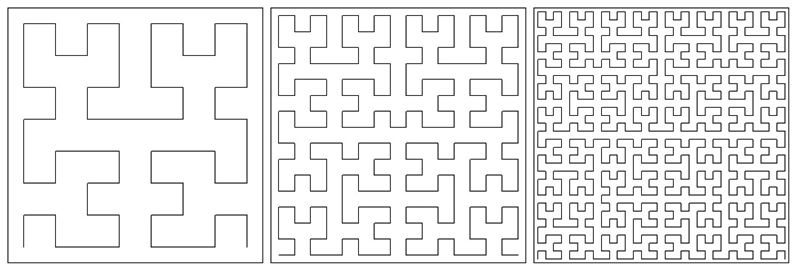
\includegraphics[width=\linewidth]{fig1}
  \caption{Examples of approximations of the Peano space-filling curves (the approximation density is equal to 2, 3 and 4 correspondingly) \cite{c5}}
  \label{fig:1}
\end{figure}

Further, in the framework of information-statistical theory, a general computational scheme of global optimization algorithms is proposed. This scheme can be summarized as follows.

Let $k$, $k \geq 2$, optimization iterations be performed, and the search information $A_k$ from (\ref{eq:13}) is obtained. To adaptively select the points of the next iterations, the optimization algorithm has to evaluate the possibility of placing the global minimum in the subintervals, into which the interval $[0,1]$ is divided by the points $x_i$, $1 \leq i \leq k$, previously performed iterations of the global search. This assessment can be performed by introducing characteristics of the subintervals, the value of which would be proportional to the degree to which the global minimum can be located in these subintervals

\begin{equation}\label{eq:15}
R(i)=\mathcal{R} (i,A_k ), 1 < i \leq k.
\end{equation}

The type of characteristics $R(i)$, $1 < i \leq k$, is a key design element of global optimization algorithms. For example, for an algorithm that builds a uniform dense grid in the search domain, the characteristics may simply be the length of the interval

\begin{equation}\label{eq:16}
R(i)=(x_i-x_{i-1}), 1 < i \leq k, \; x_i, x_{i-1} \; \mathrm{from} \; A_k.
\end{equation}

For the multidimensional generalizations of the algorithms proposed in \cite{c22,c23}, the characteristic is an estimate of the minimum possible value of the minimized function on the interval, i.e.

\begin{equation}\label{eq:17}
R(i)=0.5 H \rho_i - 0.5 (z_{i-1} + z_i), \rho_i=(x_i - x_{i-1})^{1/N}, 1 < i \leq k,
\end{equation}
where $H$ is the H\"older constant from (\ref{eq:12}) for the reduced global optimization problem to be solved; $N$ is the dimensionality of the problem from (\ref{eq:7}). For the multidimensional generalized global search algorithm (GSA) \cite{c5,c24}, developed in the framework of the information-statistical approach, the characteristic has the form

\begin{equation}\label{eq:18}
R(i)=m \rho_i+\frac{(z_i-z_{i-1})^2}{m \rho_i }-2(z_{i-1}+z_i ), \rho_i=(x_i-x_{i-1})^{1/N}  ,1 < i \leq k,
\end{equation}
where $m$ is the numerical estimate of the H\"older constant obtained from the available search information $A_k$ from (\ref{eq:13})

\begin{equation}\label{eq:19}
m=r M, M=\frac{\max|z_i-z_{i-1}|}{\rho_i}, \rho_i=(x_i-x_{i-1})^{1/N}  ,1 < i \leq k
\end{equation}
($r>1$ is the parameter of the GSA algorithm).

The presence of interval characteristics makes it possible to represent the procedure for iterating a global search as the following sequence of steps \cite{c5}.

\textit{Step 1.} Calculate the characteristics of the intervals $R(i)$, $1 < i \leq k$, and determine the interval with the maximum characteristic
\begin{equation}\label{eq:20}
R(t)=\max{R(i)}, 1 < i \leq k.
\end{equation}

\textit{Step 2.} Select the next iteration point in the interval with the maximum characteristic \footnote{The rule $X$ for choosing the point of the next iteration in the interval $(x_{t-1},x_t)$ is another design element of characteristically represented algorithms.}
\begin{equation}\label{eq:21}
x^{k+1}=X(x_{t-1},x_t ).
\end{equation}

Calculate the value $z^{k+1}$ of the minimized function at this point (the procedure for calculating the value of the function will be called a trial) and add the obtained data $(x^{k+1},z^{k+1})$ to the search information $A_k$ from (\ref{eq:13}).

\textit{Step 3.} Check the stopping condition 
\begin{equation}\label{eq:22}
\rho_t \leq \varepsilon,	
\end{equation}
where $\rho_t=(x_t-x_{t-1})^{1/N}$, $t$ from (\ref{eq:20}) and $\varepsilon > 0$ is the specified accuracy of the solution to the optimization problem. If the stopping condition (\ref{eq:22}) is reached, then the solution to the optimization problem is stopped, otherwise $k=k+1$ is assumed and the next iteration of the global search is performed. 

After the calculations are completed, the lowest calculated value of the minimized function can be taken as the global minimum estimate
\begin{equation}\label{eq:23}
z_k^*=\min{z_i}, 1 \leq i \leq k.
\end{equation}

Again, we note that the above computational scheme is quite general. Within the framework of this scheme, many global search algorithms can be presented, as evidenced, in particular, by the examples given in (\ref{eq:16})--(\ref{eq:18}), as well as other characteristically represented algorithms (see, for example, \cite{c22,c23,c24,c25,c26,c27,c28,c29,c30,c31}). Thus, the parallelization methods discussed in Section \ref{sec:4} can be used for a sufficiently wide variety of global search algorithms.

The convergence conditions for the characteristically represented algorithms depend on the properties of the interval characteristics used. For example, one of the sufficient conditions for convergence of the algorithms is the requirement that, when iterating the global search, the characteristic of the interval containing the global minimum point repeatedly takes the maximum value in Step 1 of the general characteristic scheme. This condition is fulfilled, for example, for the multidimensional generalizations of the algorithms proposed in \cite{c22,c23} for the exact setting of the H\"older constant in (\ref{eq:17}). For GSA, the sufficient condition for convergence is the relation \cite{c5}
\begin{equation}\label{eq:24}
m \geq 2H,
\end{equation}
starting with some iteration of the global search. Additional information on the convergence of characteristically represented global search algorithms can be obtained, for example, in \cite{c5}. 

In the framework of the proposed approach, the GSA algorithm described by rules (\ref{eq:18})-(\ref{eq:23}) will be used to solve global optimization problems of the set $F$. Moreover, due to the informational connectivity (\ref{eq:5}) of the problems of the set $F$, the GSA algorithm can use all the search information $A_k$ from (\ref{eq:13}) when solving the next global optimization problem. The GSA algorithm for solving problems of the set $F$ and using search information $A_k$, will be referred to as the multiple global search algorithm (MGSA). 



\section{Parallel Computations for Solving Multiple Global Optimization Problems}\label{sec:4}

In keeping with the initial assumption that it is computationally expensive to calculate the values of minimized functions of the set $F$ from (\ref{eq:3}), solving all global optimization problems (\ref{eq:1}) may require a huge amount of calculations, which increases with the number of problems to be solved. Thus, obtaining estimates of globally optimal decisions with reasonable time delays can only be achieved using parallel high-performance computational systems. 

An obvious way to apply parallel computing is to solve the problems of the set $F$ in parallel. This method is simple and does not require any additional efforts for implementation. With this approach and with a sufficient number of computational devices (cores / processors), the time needed to solve all the $F$ set will be determined by the time used in solving the most time-consuming problem. However, this time may turn out to be quite long and necessitate the use of parallel computing to solve even one global optimization problem.

Unfortunately, well-known and widely used parallelization methods are poorly applicable in the case of global optimization problems. For example, search domain distribution between processors for global optimization problems leads to the global minimum of the problems to be solved being located on only one of the processors; in this case, all other processors will perform redundant calculations.

In the framework of the information-statistical theory, a general approach to parallelizing global optimization problems has been proposed -- parallel computing is provided by parallel (simultaneous) computing of the values of the minimized function at several different points in the search domain \cite{c5}. This approach is general -- it can be applied to solving any global optimization problems in a parallel mode. And such an approach is efficient, since the most time consuming part of the problem is parallelized due to the initial assumption that calculating the values of minimized functions is computationally expensive.

Next, we propose three different ways of applying this approach for parallel solutions to multiply global optimization problems (\ref{eq:1})-(\ref{eq:3}).


\subsection{Strategy 1: The Problem-oriented Parallel Scheme} \label{subsec:1}

In this method of parallel computing, it is proposed to solve the set $F$ problems strictly sequentially, and to use all available computational resources only to solve the one optimization problem. When solving problems of the set $F$ sequentially, all available search information $A_k$, obtained in the calculation process is reused. 

To implement this approach, it is necessary to ensure that at each iteration of the global optimization problem, not one, but several points in the search domain $D$ are selected for parallel calculation of the values of the minimized function at these points. In keeping with the fact that characteristically represented global search algorithms use the characteristics of the intervals $R(i)$, $1 < i \leq k$, from (\ref{eq:15}), to assess the possibility of locating the global minimum in the subinterval of the interval $[0,1]$, it is most reasonable to select the points of the next iteration of the global search in the intervals with the maximum values of the characteristics \cite{c33,c34,c35}.

Performing iterations of a global search for a parallel generalization of the MGSA algorithm (PMGSA-1) can be represented as follows ($q>1$ is the number of available computational devices (cores/processors) with shared memory) \cite{c33,c34,c32}.

\textit{Step 1}. Calculate the characteristics of the intervals $R(i)$, $1 < i \leq k$, and determine $q$ intervals with the maximum values of characteristics 

\begin{equation}\label{eq:25}
R(t_j)=\max{R(i)},1 < i \leq k, 1 \leq j\leq q,
\end{equation}
(for $j>1$,$t_j \neq t_l$, $1 \leq l < j$ should be satisfied).

\textit{Step 2}. Select $q$ points of the next parallel iteration in the intervals with maximum characteristics

\begin{equation}\label{eq:26}
x^{k+j}=X(x_{t_j-1},x_{t_j} ), 1 \leq j \leq q,
\end{equation}
then calculate the values of $z^{k+j}$, $1 \leq j \leq q$, of the minimized function at these points and add the resulting data $(x^{k+j},z^{k+j})$, $1 \leq j \leq q$, to the search information $A_k$ from (\ref{eq:13}).

\textit{Step 3}. Check the stopping condition

\begin{equation}\label{eq:27}
\rho_{t_j} \leq \varepsilon, 1 \leq j \leq q,
\end{equation}
where $\rho_{t_j}=(x_{t_j}-x_{t_j-1} )^{1/N}$, $t_j$, $1 \leq j \leq q$, from (\ref{eq:25}) and $\varepsilon > 0$ is the specified accuracy for solving the optimization problem. If the stopping condition (\ref{eq:27}) is reached for at least one interval $t_j$, $1 \leq j \leq q$, then the solution to the optimization problem stops; otherwise $k=k+q$ is assumed and the next parallel iteration of the global search is performed. 

Results of the numerical experiments show that this approach of parallelizing the MGSA algorithm allows one to obtain near-linear speedup using up to $2^N$ computational cores ($N$ is the dimensionality of the global optimization problems to be solved). An example of using PMGSA-1 is given in Fig. \ref{fig:2}. On the left in Fig. \ref{fig:2} the MGSA result is given (55 iterations), on the right the PMGSA-1 result is shown (30 iterations, i.e., speedup is 1.8). PMGSA-1 uses 2 cores, iteration points selected by the cores are marked by the different lines.

\begin{figure}
  \centering
  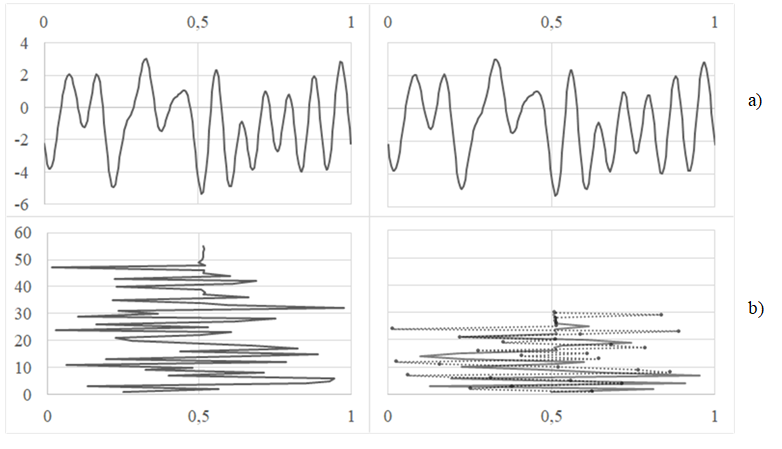
\includegraphics[width=\linewidth]{fig2}
  \caption{An example of using PMGSA-1 for solving the univariate optimization problem: a) the graph of the minimized function, b) step-by-step selection of iteration points computed by the method (the ordinate axis is the iteration number, the abscissa axis is the search domain)}
  \label{fig:2}
\end{figure}

\subsection{Strategy 2: The Competitive Parallel Scheme} \label{subsec:2}

Selecting several points at once for the same search iteration in the PMGSA-1 algorithm can result in redundant points compared to the sequential GSA version, since these points are selected at the same state of search information $A_k$ from (\ref{eq:13}). Such an undesirable effect can be reduced by reducing the number of computational devices allocated to solve an optimization problem, while simultaneously increasing the number of parallel global optimization problems that are solved due to freed computational resources. In this case, the available computational resources can be distributed dynamically among problems in the global search process.

Assume, as before, that $q>1$ is the number of available computational devices (cores/processors) with shared memory, and $ns>1$ is the number of parallel problems solved from the set $F$ from (\ref{eq:3})\footnote{Without lost of generality, we will use sequential numbering of problems solved in parallel from $1$ to $ns$.}. Each optimization problem solved in parallel will compete for available computational resources -- the distribution of resources between problems can be carried out, as before, based on the values of interval characteristics. To calculate the characteristics, the problems solved in parallel have sets of search information $A_k(j)$, $1\leq j \leq ns$, from (\ref{eq:13}), which match the set of iteration points $x_i$, $1 \leq i \leq k$, of the global search, but differ, accordingly, in the values of the minimized functions. The notation $\tau_{ij}$ will then designate the interval $t_j$ in the search information $A_k(i)$ of problem $i$.

The new parallel version of the MGSA algorithm (the PMGSA-2 algorithm) obtained as a result of this approach is determined by the following sequence of steps for performing parallel iterations of the global search.

\textit{Step 0}. For each problem to be solved in parallel, normalize the values of the minimized function in the available search information in order to compare the interval characteristics in different global optimization problems\footnote{After transformation (\ref{eq:28}), $z_k^*=0$ and $m_k=1$ are carried out for all $ns$ parallel problems.}

\begin{equation}\label{eq:28}
z(j)_i'=\frac{z(j)_i-z(j)_k^*}{m(j)_k},1 \leq i \leq k,1 \leq j \leq ns,
\end{equation}
where $z(j)_k^*$, $1 \leq j \leq ns$, are estimates (\ref{eq:23}) of the minimum values of the minimized functions, and $m(j)_k$, $1 \leq j \leq ns$, are the estimates (\ref{eq:19}) of the H\"older constant from (\ref{eq:12}). Further, when performing the steps of the algorithm, the converted values $z(j)_i'$, $1 \leq i \leq k$, $1 \leq j \leq ns$ should be used when calculating the characteristics of intervals and points of new iterations of the global search.

\textit{Step 1}. Calculate the characteristics of intervals $R(i)$, $1 < i \leq k$, for all $ns$ problems to be solved in parallel and determine $q$ intervals with the maximum values of the characteristics
\begin{equation}\label{eq:29}
R(\tau_{l(j)j})=\max{R_\nu(i)}, 1 < i \leq k, 1 \leq \nu \leq ns, 1 \leq j \leq q,
\end{equation}
where $R_\nu(i)$ is the characteristic of the interval $i$ in the search information $A_k(\nu)$ of the problem with the number $\nu$, $l(j)$ is the number of the problem to be solved, in which the maximum characteristic $R(\tau_{l(j)j})$ was chosen; (in (\ref{eq:29}) for $j>1$, $\tau_{l(j)j}\neq \tau_{l(l)l}$, $1 \leq l < j$ should be satisfied).

\textit{Step 2}. The execution of Step 2 is divided into three sequential stages: 
\begin{enumerate}
	 
	\item Select $q$ points of the next parallel iteration in intervals with maximum characteristics
\begin{equation}\label{eq:30}
 x(l(j))^{k+j}=X(x_{\tau_{l(j)j}-1},x_{\tau_{l(j)j}}),1 \leq j \leq q	
\end{equation}
(the point $x(l(j))^{k+j}$ is determined in the interval $(x_{\tau_{l(j)j}-1},x_{\tau_{l(j)j}})$, belonging to the search information $A_k (l(j))$ of problem $l(j)$.

	\item Calculate the values $z(l(j))^{k+j}$, $1 \leq j \leq q$, of minimized functions at the points $x(l(j))^{k+j}$, $1 \leq j \leq q$.
	
  \item Add the obtained data $(x(l(j))^{k+j}, z(l(j))^{k+j})$, $1 \leq j \leq q$, in the search information $A_k(i)$, $1 \leq i \leq ns$, of each problem being solved in parallel with the necessary values transformation $z(l(j))^{k+j}$, $1 \leq j \leq q$, using the $Z$ transformation from (\ref{eq:5}).

\end{enumerate}

\textit{Step 3}. Verify the stopping condition
\begin{equation}\label{eq:31}
\rho_{\tau_{l(j)j}} \leq \varepsilon, 1 \leq j \leq q,
\end{equation}
where $\rho_{\tau_{l(j)j}} = (x_{\tau_{l(j)j}} - x_{\tau_{l(j)j)-1}} )^{1/N}$, $\tau_{l(j)j}$, $1 \leq j \leq q$, from (\ref{eq:29}) and $\varepsilon > 0$ is the given accuracy for solving the optimization problem. If the stopping condition (\ref{eq:31}) is reached for at least one interval $\tau_{l(j)j}$, $1 \leq j \leq q$, then the solution to the optimization problem stops; otherwise, $k=k+q$ is assumed and the next parallel iteration of the global search is performed. 

Let us briefly explain the rules for performing a parallel iteration of the global search. The characteristics of the intervals are calculated for all $ns$ problems to be solved in parallel (Step 1), and $q$ intervals with the maximum values of the characteristics are selected among them. As a result, the available computational resources are distributed dynamically among problems -- computational devices can be distributed evenly between problems, or they can be allocated to only one problem with the best interval characteristics. After calculating the values of the minimized functions (Step 2), the new search data obtained is added to the search information of all solved problems; regardless of where the intervals for iterating the global search were selected, the search information of all solved problems is updated with a full set of new search data.

The maximum efficiency of the proposed PMGSA-2 algorithm is achieved if the global minimum in parallel problems is reached at the same point in the search domain. In any case, getting additional search information from simultaneously solved problems can significantly reduce the time needed to solve each global search problem -- see the results of numerical experiments in Section \ref{sec:5}. An example how PMGSA-2 selects the intervals with the maximum characteristics (Step 1) is given in Fig.\ref{fig:3}.

\begin{figure}
  \centering
  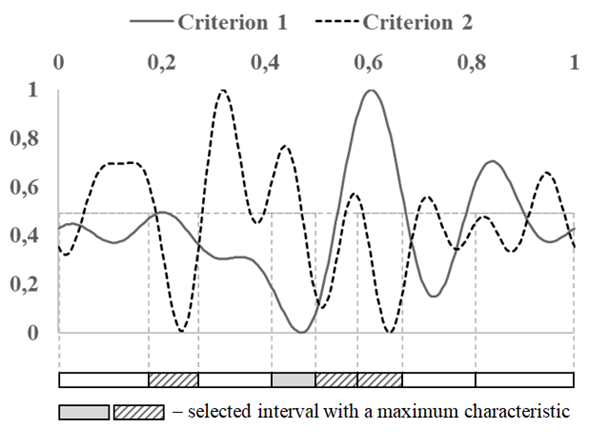
\includegraphics[width=0.7\linewidth]{fig3}
  \caption{An example of intervals selection by the PMGSA-2 algorithm (Step 1)}
  \label{fig:3}
\end{figure}

\subsection{Strategy 3: The Cooperative Parallel Scheme} \label{subsec:3}

When using computational devices with shared memory, the number of cores / processors is quite limited -- the number of processors on one computational node is usually 2, the number of computational cores in one processor usually does not exceed 10-20. For increasing possible parallelism, it becomes inevitable to use computational nodes where memory is distributed.

Let $p>1$ be the number of computational nodes with distributed memory, each of which has $q>1$ computational cores (that is, the total number of cores in a computational system is $p*q$). 

In the framework of the proposed approach, a parallel multiple search algorithm (the PMGAS-3 algorithm) is proposed for distributed memory computational systems, the main rules of which are as follows.

1) Solving the problems of the set $F$ from (\ref{eq:3}) is carried out sequentially in groups; the number of problems in each group coincides with the number of available computational nodes.

2) Each problem of the current group is solved on its own computational node using the PMGSA-1 algorithm.

At the end of each parallel iteration of the global search, the results of the iteration $(x^{k+j}, z^{k+j})$, $1 \leq j \leq q$, of each processor are transferred to all available nodes of the computational system with the necessary transformation of the values of minimized functions in accordance with the transformation $Z$ from (\ref{eq:5}).
		
Before performing a new iteration, each computational node accepts the search data transmitted to it and adds this data to the search information $A_k$ from (\ref{eq:13}).
	
In this way, in keeping with the above rules, the PMGSA-3 algorithm is distributed -- the problems of the set $F$ are solved independently on different computational nodes. During the global search process, computational nodes exchange the calculation results that are obtained; after each iteration of the global search, the search information for each problem being solved is updated with $q$ calculated values of the minimized function. Thus, the more computational nodes there are (and accordingly, simultaneously solved problems), the faster as a rule, each optimization problem is solved. This is evidenced, in particular, by the results of numerical experiments that were performed (see Section \ref{eq:5}). An example how PMGSA-3 performs an optimization iteration is given in Fig. \ref{fig:4}.

\begin{figure}
  \centering
  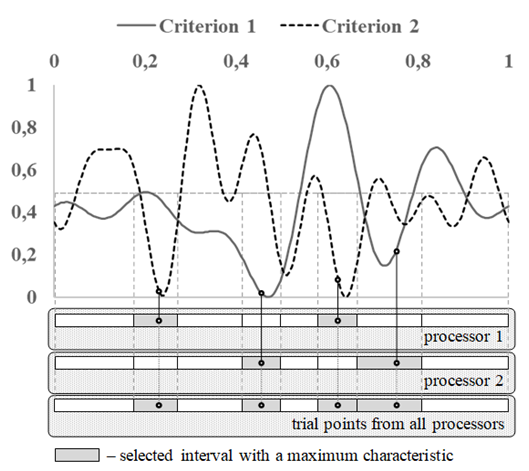
\includegraphics[width=0.7\linewidth]{fig4}
  \caption{Intervals and trial points selected by the PMGSA-3 algorithm}
  \label{fig:4}
\end{figure}

\section{Results of Numerical Experiments}\label{sec:5}

Numerical experiments were performed on the supercomputers Lobachevsky (University of Nizhni Novgorod), Lomonosov (Moscow State University), MVS-10P (Joint Supercomputer Center of RAS) and supercomputers Endeavor. The numerical results were obtained by using the following computational nodes: 2 Intel Xeon Platinum 8260L, 2.4 GHz, 256 GB RAM (i.e. a total of 48 CPU cores were available on each node). The executable program code was built by using the Intel Parallel Studio XE 2019 software package. The numerical experiments were performed using the Globalizer system \cite{c40}.

First, we present the results achieved when comparing the MGSA algorithm with several multicriteria optimization algorithms \cite{c37}. In carrying out the experiments, the two-criteria test problem proposed in \cite{c36} was used:

\begin{equation}\label{eq:32}
f_1(y)=(y_1-1) y_2^2+1,f_2 (y)=y_2, 0 \leq y_1, y_2 \leq 1.
\end{equation}

Solving the MCO problem is understood to mean the construction of a numerical approximation of the Pareto domain. To assess the quality of the approximation, the completeness and uniformity of coverage of the Pareto domain were compared using the following two indicators \cite{c15,c36}:
\begin{itemize}
	 \item The hypervolume index (HV). This indicator characterizes how completely the Pareto domain is approximated (a higher value corresponds to a more complete coverage of the Pareto domain). 
	 \item The distribution uniformity index (DU). This indicator characterizes how uniformly the Pareto domain is covered (a lower value corresponds to a more uniform coverage of the Pareto domain).
\end{itemize}

During the experiments, five multicriteria optimization algorithms were compared: the Monte-Carlo (MC) method, the genetic algorithm SEMO from the PISA library \cite{c37,c38}, the Non-uniform coverage (NUC) method \cite{c36}, the bi-objective Lipschitz optimization (BLO) method \cite{c37} and the MGSA algorithm. For the MGSA  algorithm, 50 subproblems $G(\lambda, y)$ from (\ref{eq:32}) were solved for different values of convolution coefficients $\lambda$, uniformly distributed in the interval $[0,1]$. The results of the experiments are presented in Table \ref{tab:1}.

\begin{table}[ht]
\centering
\caption{Comparison of the effectiveness of multicriteria optimization algorithms \cite{c37})}
\label{tab:1}
\begin{tabular}{cccccc}
\hline
Method                                                                                     & MC    & SEMO  & NUC   & BLO   & \textbf{MGSA} \\ \hline
Iteration number                                          & 500   & 500   & 515   & 498   & \textbf{370}   \\
\begin{tabular}[c]{@{}c@{}}Number of Pareto optimal points\end{tabular} & 67    & 104   & 29    & 68    & \textbf{100}    \\
HV                                                        & 0.300 & 0.312 & 0.306 & 0.308 & \textbf{0.316} \\
DU                                                        & 1.277 & 1.116 & 0.210 & 0.175 & \textbf{0.101} \\ \hline
\end{tabular}
\end{table}

These numerical results show that the MGSA algorithm has a noticeable advantage in almost all performance indicators when compared with the methods of multicriteria optimization being considered, even when solving relatively simple MCO problems.

Further the numerical experiments were performed for evaluating the efficiency of the parallel PMGSA-1,2,3 algorithms in solving the MGO problems. In the experiments, the MGO problems were generated as problems seeking a set of efficient solutions to the MCO problems using the minimax convolution $G (\lambda, y)$ from (\ref{eq:7}) for different values of the convolution coefficients $\lambda$, uniformly distributed in the domain $\Lambda$. Given the initial assumption about the high complexity of computing the values of minimized functions of the set $F$ from (\ref{eq:3}), the efficiency of the proposed methods is evaluated by the number of optimization iterations performed by the methods to achieve the required accuracy under the stopping condition from (\ref{eq:22}).

In the first series of numerical experiments, five-criteria four-dimensional MCO problems were solved, i.e. $N = 4$, $m = 5$. In the experiments, 100 MCO problems were solved, in which multiextremal functions obtained by using the GKLS generator \cite{c39} were used as the efficiency criteria; for each problem 100 efficient solutions were calculated (i.e., a total of $10,000$ subproblems $G (\lambda, y)$ were solved). The results obtained (the number of search iterations performed before the stopping condition was fulfilled) were averaged out over the number of MCO problems solved. In solving the problems, the search accuracy $\varepsilon = 0.05$ from (\ref{eq:22}) and the reliability of the method $r = 5.6$ from (\ref{eq:19}) were used.
 
The results of the numerical experiments are presented in Table \ref{tab:2}. The first three rows of the table contain information about the computational resources used during the experiments. The first row marked as ``$p$'' indicates the number of computational nodes used. The number of cores used within a single node is presented in the second row marked as ``$q$''. The total number of cores used is presented in the third row marked as ``$p*q$''. The rows four through six show the average number of iterations performed by PMGSA-1,2,3 for solving a single MCO problem accordingly.

\begin{table}[ht]
\centering
\caption{The results of a series of experiments to solve five-criteria four-dimensional MCO problems}
\label{tab:2}
\begin{adjustbox}{max width=\textwidth}
\begin{tabular}{cccccccc}
\hline
\multicolumn{8}{c}{Computational resources used}                                                                                                                           \\ \hline
p                   & 1                     & 1                   & 1                  & 1                  & 2                  & 5                  & 10                 \\
q                   & 1                     & 5                   & 25                 & 48                 & 48                 & 48                 & 48                 \\
p*q                 & 1                     & 5                   & 25                 & 48                 & 96                 & 240                & 480                \\ \hline
\multicolumn{8}{c}{Average number of iterations for solving one   MCO problem}                                                                                             \\ \hline
PMGSA-1             & 117,490.8             & 19,586.9            & 4,232.4            & 2,116.5            & -                  & -                  & -                  \\
PMGSA-2             & 130,027.1             & 20,002.0            & 4,320.1            & 2,160.7            & -                  & -                  & -                  \\
PMGSA-3             & 117,490.8             & 19,586.9            & 4,232.4            & 2,116.5            & 1,064.6            & 534.3              & 285.5              \\ \hline
\multicolumn{8}{c}{Speedup obtained by using parallel methods}                                                                                                             \\ \hline
PMGSA-1             & 1                     & 6.0                 & 27.8               & 55.5               & -                  & -                  & -                  \\
PMGSA-2             & 1                     & 6.5                 & 30.1               & 60.2               & -                  & -                  & -                  \\
PMGSA-3             & 1                     & 6.0                 & 27.8               & 55.5               & 110.4              & 219.9              & 411.5              \\ \hline
\multicolumn{8}{c}{\begin{tabular}[c]{@{}c@{}}Overall reduction of executed iterations provided   \\ by parallel computations and reusing search information\end{tabular}} \\ \hline
PMGSA-1             & 11.9                  & 71.3                & 330.0              & 659.9              & -                  & -                  & -                  \\
PMGSA-2             & 10.7                  & 69.8                & 323.3              & 646.5              & -                  & -                  & -                  \\
PMGSA-3             & 11.9                  & 71.3                & 330.0              & 659.9              & 1,312.0            & 2,614.4            & 4,892.5            \\ \hline
\end{tabular}
\end{adjustbox}
\end{table}

It should be noted that for the initial sequential GSA algorithm without reusing search information, an average of 1,396,804.1 iterations are required to solve a single MCO problem. The overall reduction of the number of executed iterations, taking into account the effect of reusing search information, is indicated in the last three rows of Table \ref{tab:2}.

\begin{figure}
  \centering
  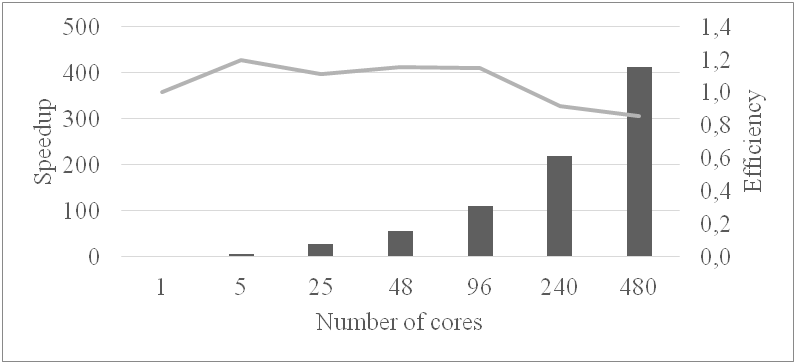
\includegraphics[width=0.7\linewidth]{fig5}
  \caption{Speedup and efficiency of the PMGSA-3 algorithm in solving five-criteria four-dimensional MKO problems}
  \label{fig:5}
\end{figure}


It follows from the results of the experiments (see also Fig. \ref{fig:5}), that the proposed parallel methods provide superlinear speedup\footnote{Superlinear speedup can be achieved due to the fact that the sets of iteration points that are selected when performing iterations of the global search by sequential and parallel algorithms are not identical (the search information of the methods may differ).} and high scalability (maintaining the efficiency of parallel computing with an increase in the number of computational cores used). When using a single computational node and all available computational cores for shared memory computational systems, the computational speedup exceeds 55 (with 48 computational cores in use). When using 10 computational nodes (480 cores) with distributed memory, the speedup becomes 411.5. Taking into account the effect of search information reuse, the overall reduction of the number of global optimization iterations is more than 4,890 times.

In the second series of the experiments, the problems being solved were made more complicated by increasing the dimensionality -- the five-criterion six-dimensional MCO problem was solved, i.e., $N = 6$, $m = 5$. For solving these problems the parallel PMGSA-3 method was applied. When performing the experiments, the accuracy of the method $\varepsilon = 0.1$ from (\ref{eq:22}) and the reliability of the method $r = 5.6$ were used. The results of the experiments are presented in Table \ref{tab:3}.

The first three rows of the table, as before, present the number of computational nodes used, the number of cores per a node and the total number of computational cores. The last three rows correspond to the number of global search iterations performed, the speedup achieved, and the overall reduction of executed iterations, taking into account the reuse of information (the average number of iterations performed by the sequential GSA algorithm without the reuse of search information for solving one MCO problem is, on average, 3,131,284.8).
Based on the results of the experiments, it can be seen that when the dimensionality of the problem is increased, the efficiency of parallel computations using the PMGSA-3 algorithm also increases (when using 480 cores, the speedup is 472.9). Taking into account the effect of search information reuse, the number of global optimization iterations is reduced, in total, by more than 4,160 times.

\begin{table}[ht]
\centering
\caption{Results of experiments to solve the five-criterion six-dimensional MCO problem using the parallel PMGSA-3 method}
\label{tab:3}
\begin{adjustbox}{max width=\textwidth}
\begin{tabular}{ccccccc}
\hline
\multicolumn{7}{c}{Computational resources used}                                                                                                  \\ \hline
p                                                                                & 1         & 1        & 1        & 1        & 5       & 10      \\
q                                                                                & 1         & 5        & 25       & 48       & 48      & 48      \\
p*q                                                                              & 1         & 5        & 25       & 48       & 240     & 480     \\ \hline
\multicolumn{7}{c}{Results of numerical experiments}                                                                                              \\ \hline
Iterations                                                                       & 364,713.2 & 97,387.5 & 19,791.0 & 11,294.0 & 1,561.2 & 771.2   \\
Speedup                                                                          & 1         & 3.7      & 18.4     & 32.3     & 233.6   & 472.9   \\
\begin{tabular}[c]{@{}c@{}}Overall reduction \\ of iteration number\end{tabular} & 8.6       & 32.2     & 159.6    & 277.5    & 2,025.6 & 4,160.1 \\ \hline
\end{tabular}
\end{adjustbox}
\end{table}


\section{Conclusion}\label{sec:6}

The paper considers a new class of optimization problems -- multiple global optimization problems, in which minimized functions can be multiextremal, and calculating function values may require a huge amount of calculations. In addition, the set of problems to be solved can change dynamically during calculations by adding or removing solvable global optimization problems. Problems of this kind are encountered, for example, when it is necessary to find several efficient solutions of multicriteria optimization problems or when part of the variable parameters of optimization problems can take only a number of discrete values. Problems of this class have a high computational complexity and the ability to solve such problems efficiently can be achieved only by using high-performance computational systems.

The proposed approach assumes that information connectivity exists in the global optimization problems being solved, when the calculated values of any function of the set of problems to be solved can be transformed to the values of any other functions without time consuming calculations. In such cases, all the search information obtained in solving a particular optimization problem can be used to solve all the other problems. Such reuse of search information can significantly reduce the amount of calculations performed, up to just a few iterations when solving the next problems of multiple global optimization.

The availability of informational connectivity significantly expands the possibilities of parallel solutions of the entire set of multiple global optimization problems. The paper proposes two parallel computational schemes: a cooperative scheme, when several problems are solved simultaneously, with the search information that is obtained being exchanged between problems, and a competitive scheme, when problems that are simultaneously being solved compete with each other for using the available computational resources.

Results of computational experiments show that the proposed approach allows us to significantly -- by tens and hundreds of times -- reduce the computational complexity of solving multiple global optimization problems.
In general, one can observe that the proposed approach is promising and requires further research. First, continued computational experiments must be carried out to solve the problems of multiple global optimization of varying computational complexity. It is also necessary to assess the possibility of using other global optimization algorithms within the framework of the proposed approach.

\section*{Acknowledgements} 
This research was supported by the Russian Science Foundation, project No 16-11-10150 ``Novel efficient methods and software tools for time-consuming decision making problems using supercomputers of superior performance''

\biboptions{sort&compress}
\bibliography{mybibfile}


\end{document}